\documentclass{article}
\usepackage[margin=1in]{geometry}
\usepackage{fancyhdr}
\usepackage{graphicx}
\usepackage{amsmath}
\usepackage{cancel}
\usepackage{caption}
\usepackage{nccmath}
\graphicspath{ {images/} }

\pagestyle{fancy}
\lhead{BME 384}
\rhead{Pascale Walters 20566177\\
		Lee Yu Wu 20558313}

\begin{document}

\begin{center}\underline{\huge Hands-On Fluids Challenge}\end{center}

\begin{abstract}
Hello
\end{abstract} 

\section{Theoretical Calculation}
%
The first objective of the experiment is to model the height of the jet as a function of the speed of the displacement of the piston of the syringe. This is accomplished by defining a relationship between the velocity of the fluid leaving the tip of the needle at \textcircled{2} and the velocity of the fluid at the highest point of the jet stream at \textcircled{3} through the mass balance equation and Bernoulli's Principle. These locations are illustrated in Figure \ref{fig:1}.

%
\begin{figure}[h!]
\centering
  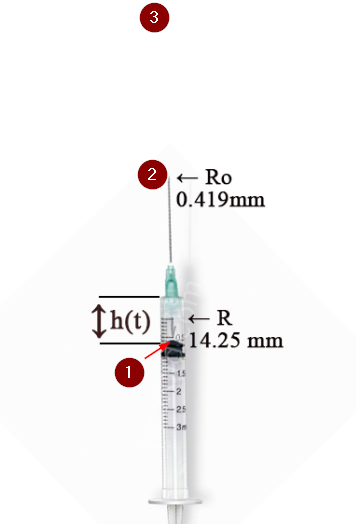
\includegraphics[width=50mm]{Syringe.png}
  \captionsetup{justification=centering}
  \caption{An illustration of the syringe. The label points are used in mass balance and Bernoulli.}
  \label{fig:1}
\end{figure}
%
From the mass balance equation,
\begin{align*}
0= \frac{\partial}{\partial{t}} \int_{cv} \rho dv + \int_{cs} \rho \bar{v} \cdot d\bar{A} \label{eq:1} 
\end{align*} 

The control volume consists of the entire syringe (i.e. all volumes enclosed between \textcircled{1} and \textcircled{2}). As there is fluid existing the control volume, $\frac{\partial}{\partial{t}} \int_{cv} \rho dv$ is non zero. Integrating the two terms shown in \eqref{eq:1} yields the following results:

\begin{align*}
\frac{\partial}{\partial{t}} \int_{cv} \rho dv = \frac{dm}{dt}
\end{align*}
\begin{align*}
\int_{cs} \rho \bar{v} \cdot d\bar{A} = \rho \bar{v_2} \pi R_o^2
\end{align*}

Substituting the individual terms into \eqref{eq:1} results in
\begin{align*}
\frac{dm}{dt} = - \rho \bar{v_2} \pi R_o^2
\end{align*}
\begin{align*}
\rho \pi R^2 \frac{dh}{dt} = \rho \pi \bar{v_2} R_o^2
\end{align*}
Since the jet stream is a free jet, the velocity profile can be assumed to be uniform and therefore, $\bar{v_2} = v_2$.
\begin{align*}
\frac{dh}{dt} = -(\frac{R_o}{R})^2 v_2
\end{align*}
\begin{align}
v_2 = -\frac{dh}{dt} (\frac{R}{R_o})^2
\end{align}

The highest point of the jet stream (i.e. \textcircled{3}) is related to the exist velocity at \textcircled{2} by Bernoulli's Principle.
\begin{align*}
\frac{P_2}{\rho} + g z_2 + \frac{\alpha v_2^2}{2} = \frac{P_3}{\rho} + g z_3 + \frac{\alpha v_3^2}{2} 
\end{align*}
Taking $z_2$ as the reference point reduces the term to zero and the velocity at the highest point is also zero.
\begin{align}
\frac{P_2}{\rho} + g \cancelto{0}{z_2} + \frac{\alpha v_2^2}{2} = \frac{P_3}{\rho} + g z_3 + \frac{\alpha \cancelto{0}{v_3^2}}{2} \label{eq:2}  
\end{align}
where
\begin{align*}
P_2 = P_atm + P_c
\end{align*}
\begin{align*}
P_c = \frac{2\gamma}{d} = \frac{2\gamma}{2 R_o} = \frac{\gamma}{R_o}  \textrm{ and } \gamma = 72 \frac{mN}{m}  \textrm{ for air-water interface}
\end{align*}
and 
\begin{align*}
\alpha = 2 \textrm{ for laminar flow as shown by experimental calculation}
\end{align*}
Substituting \eqref{eq:1} back to \eqref{eq:2}:
\begin{align*}
z_3 = \frac{1}{g} (\frac{\gamma}{R_o \rho} + (\frac{dh}{dt})^2(\frac{R}{R_o})^4)  
\end{align*}
where $z_3$ is the highest point the jet stream can reach in meters.

\begin{multline*}
z_3 = \frac{1}{9.81} (\frac{72\times10^{-3}}{0.419\times10^{-3} \times 1000} + (\frac{dh}{dt})^2(\frac{14.25\times10^{-3}}{0.419\times10^{-3}})^4)\\= 0.102\times(0.172 + (\frac{dh}{dt})^2 \times1.34\times{10^6}) \textrm{ where $\frac{dh}{dt}$ varies in each experiment}
\end{multline*}

\section{Discussion}

\setlength{\parindent}{1cm} 
\end{document}